\section{Results}

This was moderately easy to program and we also had \href{https://github.com/tatha04/Numerical-Renormalization-Group}{this code} as a reference to ensure bugs were avoided. We chose to keep $N_s = 1000$ states each iteration\footnote{This is a very large number when you consider we are attempting to diagonalize 1000$\times$1000 matrices. Evidently, both computing efficiency and our symmetry considerations are very powerful.}, and we picked $\Lambda=3.0$ and do 70 iterations. We also chose two sets of values for $\epsilon_f$, $U$, and $V$, corresponding to the impurity occupation energy, the impurity onsite repulsion $U$, and hybridization $V$. For both, we set $2\epsilon_f + U = 0$; this choice is often called the \textit{symmetric Anderson model}. $V$ was kept fixed at $\num{4d-4}$, and $U$ was set to $\num{d-3}$ and $\num{d-2}$.


\subsection{Energy Flows}

\begin{figure}
  \centering
  \begin{subfigure}[b]{0.4\linewidth}
    \centering
    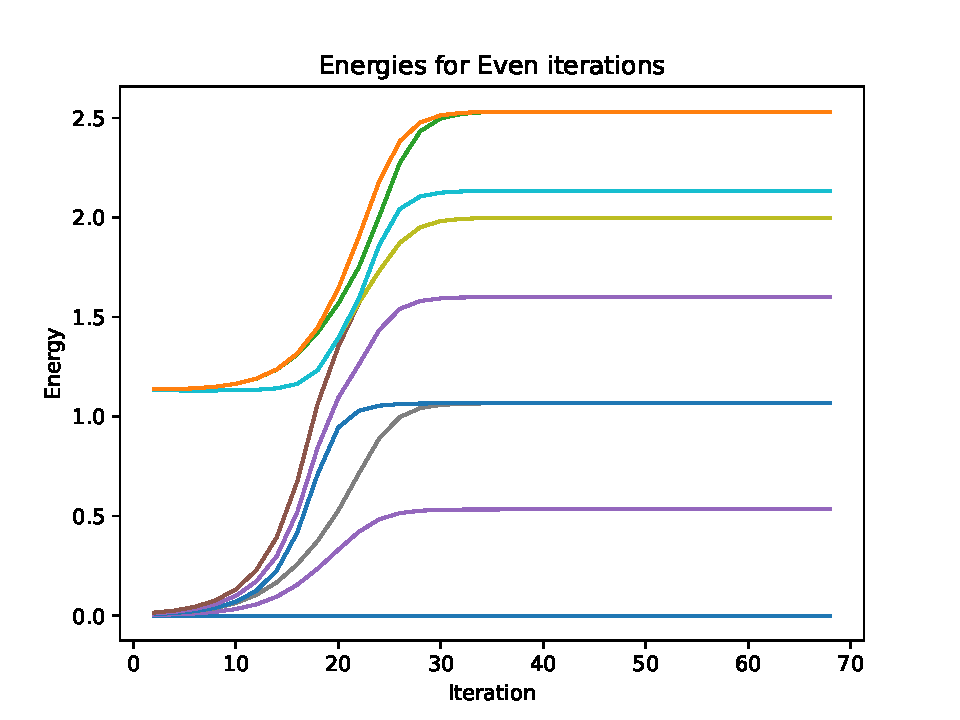
\includegraphics[width=\linewidth]{./gfx/results/even_lowU.pdf}
    \caption{Even iterations.}
    \label{fig:5-results-energies-lowu-a}
  \end{subfigure}
  \begin{subfigure}[b]{0.4\linewidth}
    \centering
    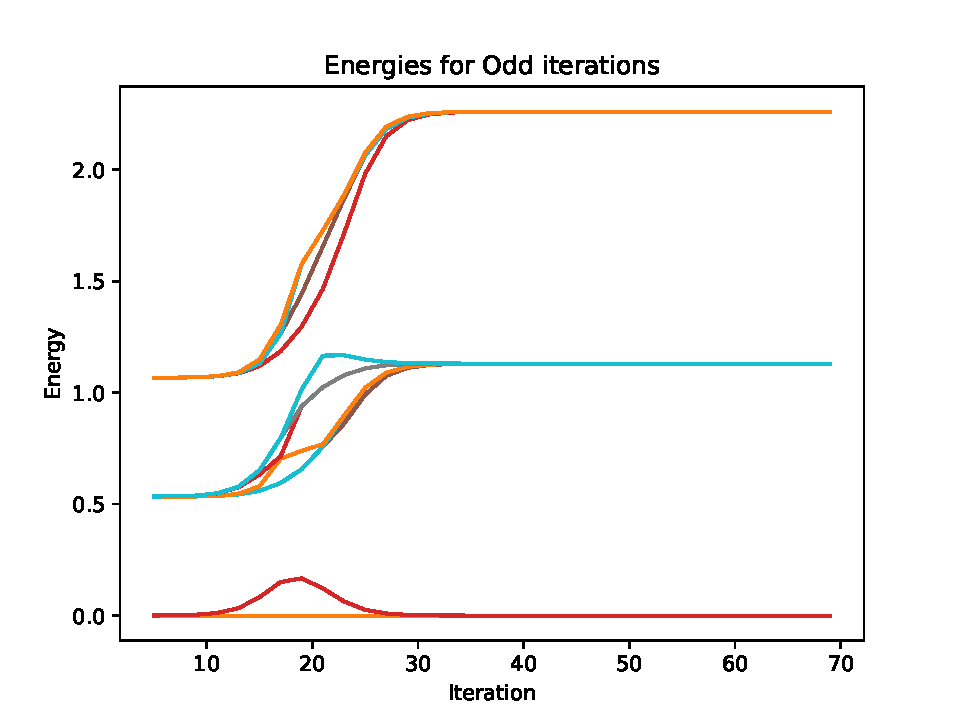
\includegraphics[width=\linewidth]{./gfx/results/odd_lowU.pdf}
    \caption{Odd iterations.}
    \label{fig:5-results-energies-lowu-b}
  \end{subfigure}
  \caption{Energy flows for $\abs{U} \sim V$.}
\end{figure}

In Figs.~\ref{fig:5-results-energies-lowu-a} and~\ref{fig:5-results-energies-lowu-b} are the energy flows for the case where we took $\abs{2\epsilon_f} \sim \abs{U} \sim V$, i.e. we set all variables roughly equivalent. One important to notice is that there is a crossover at around 18 iterations between stable flows. This is related to the fixed points described in Sec.~\ref{sec:5-nrg-renormgroup}; lower iterations correspond to higher temperatures, so the stability observed in the first 18 iterations is related to the fact that at high energies, thermal fluctuations and other effects dominate over anything related to the impurity: it's just a free moment. However, right at the point where the singlet begins to form, we have the crossover to another fixed point related to the very large coupling limit where we have the singlet.

\begin{figure}
  \centering
  \begin{subfigure}[b]{0.4\linewidth}
    \centering
    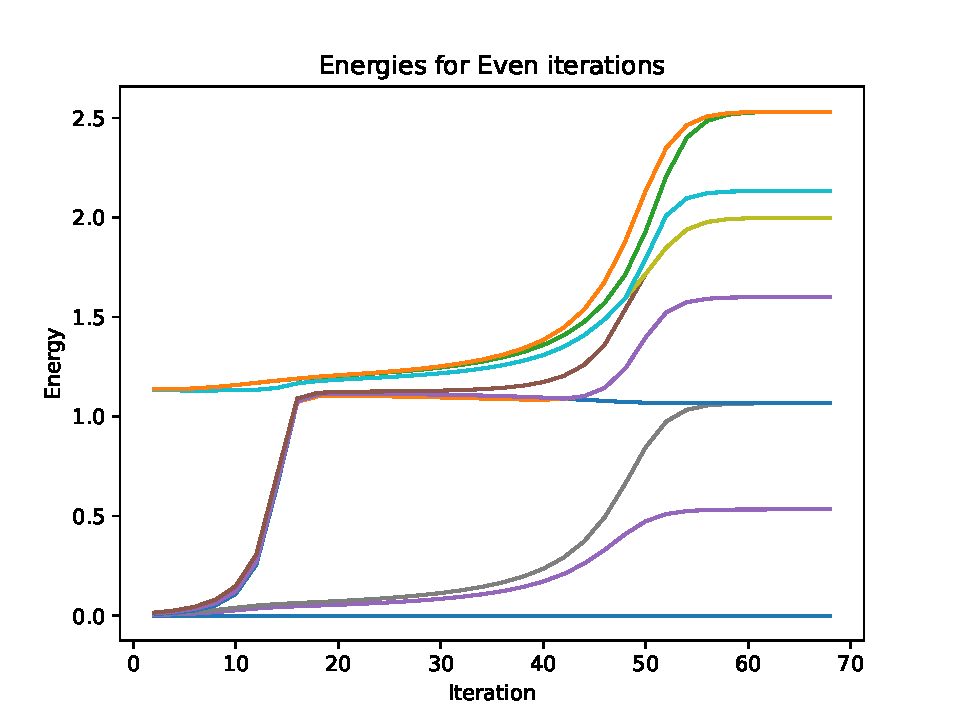
\includegraphics[width=\linewidth]{./gfx/results/even.pdf}
    \caption{Even iterations.}
    \label{fig:5-results-energies-a}
  \end{subfigure}
  \begin{subfigure}[b]{0.4\linewidth}
    \centering
    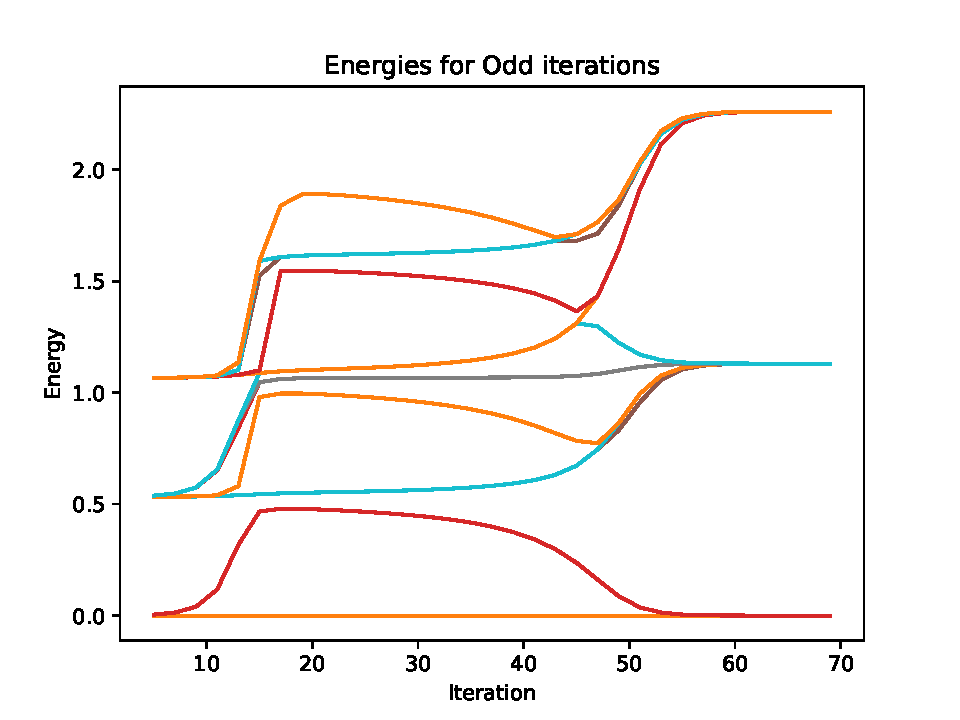
\includegraphics[width=\linewidth]{./gfx/results/odd.pdf}
    \caption{Odd iterations.}
    \label{fig:5-results-energies-b}
  \end{subfigure}
  \caption{Energy flows for $\abs{U} \gg V$}
\end{figure}

To explore this further, we took $U$ to be 10 times larger, and the results are given in Figs.~\ref{fig:5-results-energies-a} and~\ref{fig:5-results-energies-b}. This time we have two crossovers; the first one no longer is related to the crossover directly to the singlet, but rather a weakly coupled local moment, where due to the high repulsion and occupation energy, it's a bit harder to kick a conduction electron from the Fermi sea to form the bound state. After a while, though, we do notice this occur since we have the second crossover. We notice this behavior with all of the thermodynamic quantities, too.

\subsection{Magnetic Susceptibility}

Before looking at the magnetic susceptibility flows, we want to make sure we retrieve what we expect to retrieve. In particular, we know that the form of the magnetic susceptibility goes like\footnote{See Ref.~\cite{Hewson_1993}, for instance.}

\begin{equation}
  \chi_{\mathrm{imp}}(T) = \frac{(g\upsilon_B)^2}{4K_B T[1 + \exp(-U/2k_B T)]},
\end{equation}

or, taking $(g\upsilon_B) \rightarrow 1$ to go unitless, we have

\begin{equation}
  k_B T \chi_{\mathrm{imp}}(T) = \frac{1}{4(1 + e^{-U/2k_B T})}.\label{eq:5-results-tchi}
\end{equation}

We can notice immediately that in the high temperature limit where $T \gg U$, we would have the susceptibility approach $k_B T \chi_{\mathrm{imp}}(T) \rightarrow 1/8$, and in the other limit we would expect it to vanish; this is exactly what we observe, if we examine Figs.~\ref{fig:5-results-tchi-lowu} and~\ref{fig:5-results-tchi}. This is also physically what we expect: in the high coupling limit, the induced spin density fully compensates the spin of the singlet, so there should be no residual spin/magnetization remaining.

\begin{figure}
  \centering
  \begin{subfigure}[b]{0.4\linewidth}
    \centering
    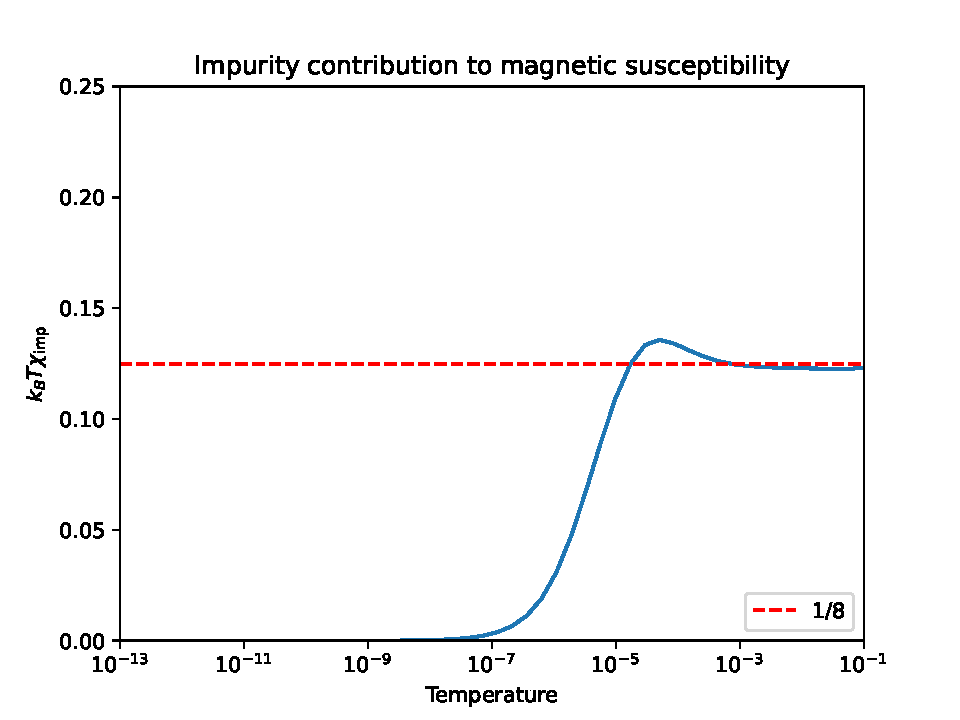
\includegraphics[width=\linewidth]{./gfx/results/tchi_lowU.pdf}
    \caption{Magnetic susceptibility flow for $\abs{U} \sim V$.}
    \label{fig:5-results-tchi-lowu}
  \end{subfigure}
  \begin{subfigure}[b]{0.4\linewidth}
    \centering
    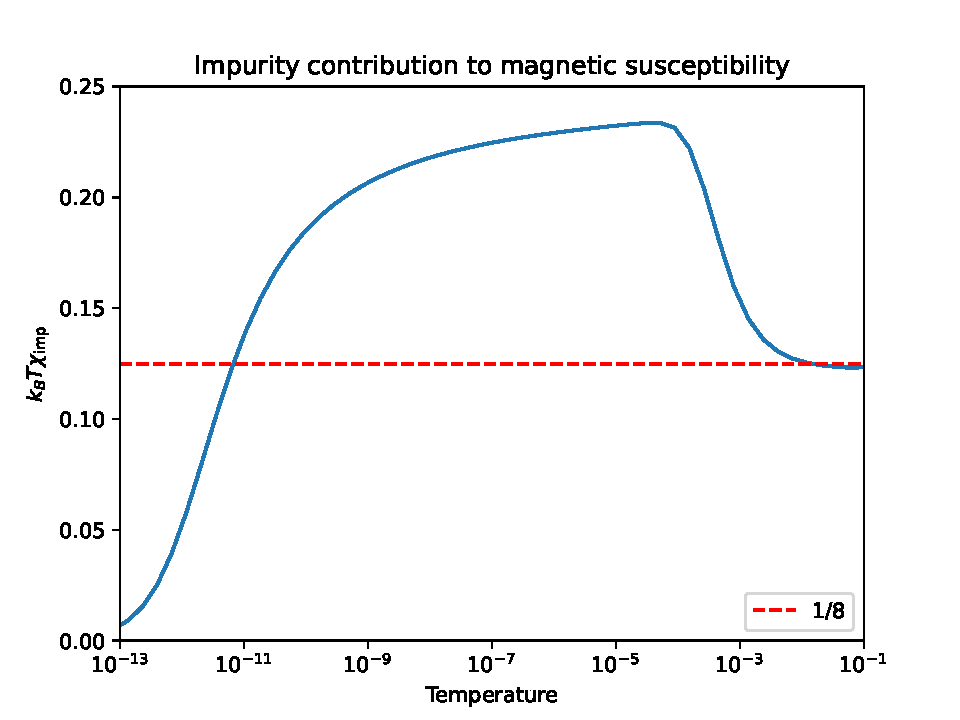
\includegraphics[width=\linewidth]{./gfx/results/tchi.pdf}
    \caption{Magnetic susceptibility flow for $\abs{U} \gg V$.}
    \label{fig:5-results-tchi}
  \end{subfigure}
\end{figure}

Interestingly, we notice the same crossover points as with the energy flows. Fig.~\ref{fig:5-results-tchi-lowu} is the plot for $\abs{U} \sim V$, where there is only one crossover between the free moment and the strongly coupled singlet. However, in Fig.~\ref{fig:5-results-tchi}, where $U$ was taken to be 10 times larger, we notice the second crossover. In the limit for strong $U$, we would have, from Eq.~\eqref{eq:5-results-tchi}, that $k_B T \chi_{\mathrm{imp}} \approx 1/4$ for this region, which is close to what we found. It would be tough to get exactly $1/4$ since at this scale we don't necessarily have $U \gg T$, meaning the exponential isn't vanishingly small, but we can see that it is close and reproduces what we expect.


\subsection{Entropy}

In the case of entropy, we know that it has the form $S = k_B \ln\Omega$, where $\Omega$ is the multiplicity of the system. In our case, we can first easily note that in the case of the singlet, there is really only one possible way to organize the system. Therefore, the multiplicity is 1 so $S = k_B \ln 1 = 0$, which is what we observe in Figs.~\ref{fig:5-results-s-lowu} and~\ref{fig:5-results-s}. Further, in the free local moment, there should be 2 ways to organize that, either a spin up or spin down, meaning we would expect it to go like $\ln2$, which it also does.

\begin{figure}
  \centering
  \begin{subfigure}[b]{0.4\linewidth}
    \centering
    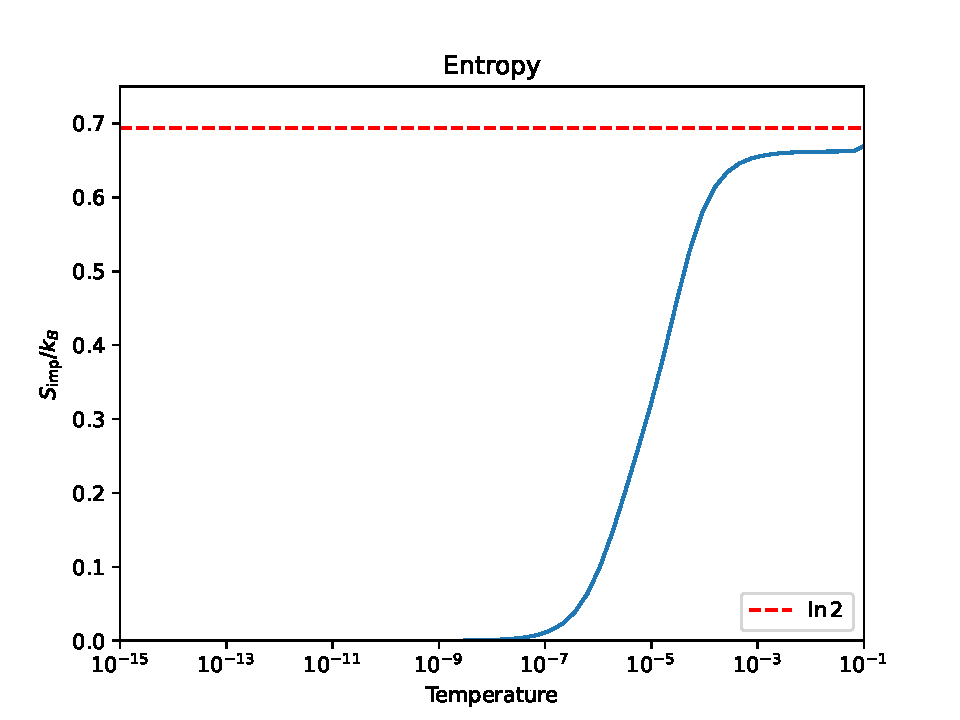
\includegraphics[width=\linewidth]{./gfx/results/s_lowU.pdf}
    \caption{Entropy flow for $(2\epsilon_f = -U) \sim V$.}
    \label{fig:5-results-s-lowu}
  \end{subfigure}
  \begin{subfigure}[b]{0.4\linewidth}
    \centering
    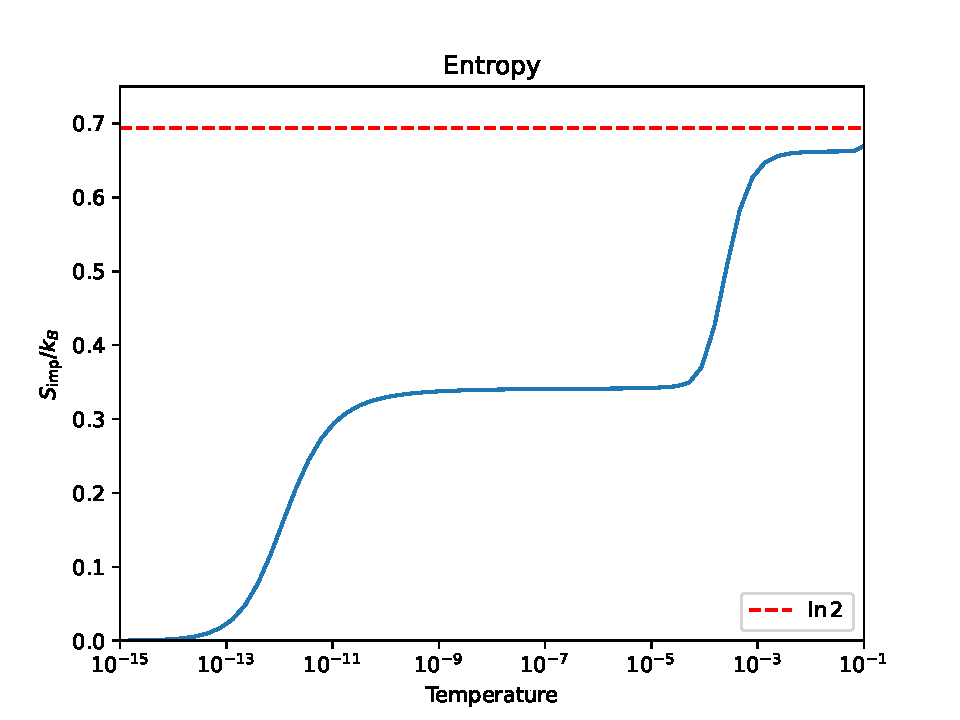
\includegraphics[width=\linewidth]{./gfx/results/s.pdf}
    \caption{Entropy flow for $(2\epsilon_f = -U) \gg V$.}
    \label{fig:5-results-s}
  \end{subfigure}
\end{figure}

Further, just as with the energy flows and magnetic susceptibility, we notice the appearance of the weakly coupled local moment fixed point for large $U$. Unfortunately, my knowledge of thermal physics and statistical mechanics is a little lacking to explain the exact reason for an apparently non-integer multiplicity, but it is good that there is still the appearance of this fixed point, it further solidifies the fact that there is a weakly coupled local moment in the high $U$ case.

\subsection{Heat Capacity}

For the heat capacity, we expect for the contribution from the impurity to vanish in both limits, i.e. when it is both a perfectly free moment and when it is a Kondo singlet. We also notice that are peaks at the crossover points; wo find one peak in the $\abs{U} \sim V$ case as in Fig.~\ref{fig:5-results-cv-lowu} and two peaks in the large $U$ case as in Fig.~\ref{fig:5-results-cv}. Unfortunately, again, I do not know enough to explain the behavior apart from this.

\begin{figure}
  \centering
  \begin{subfigure}[b]{0.4\linewidth}
    \centering
    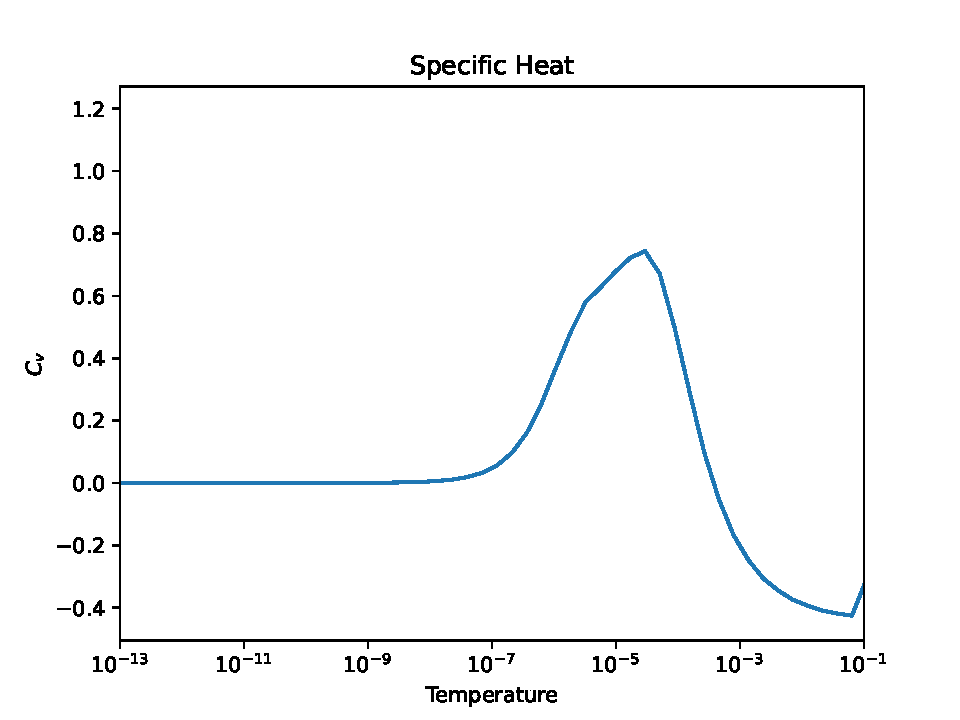
\includegraphics[width=\linewidth]{./gfx/results/Cv_lowU.pdf}
    \caption{Flow of heat capacity for $(2\epsilon_f = -U) \sim V$.}
    \label{fig:5-results-cv-lowu}
  \end{subfigure}
  \begin{subfigure}[b]{0.4\linewidth}
    \centering
    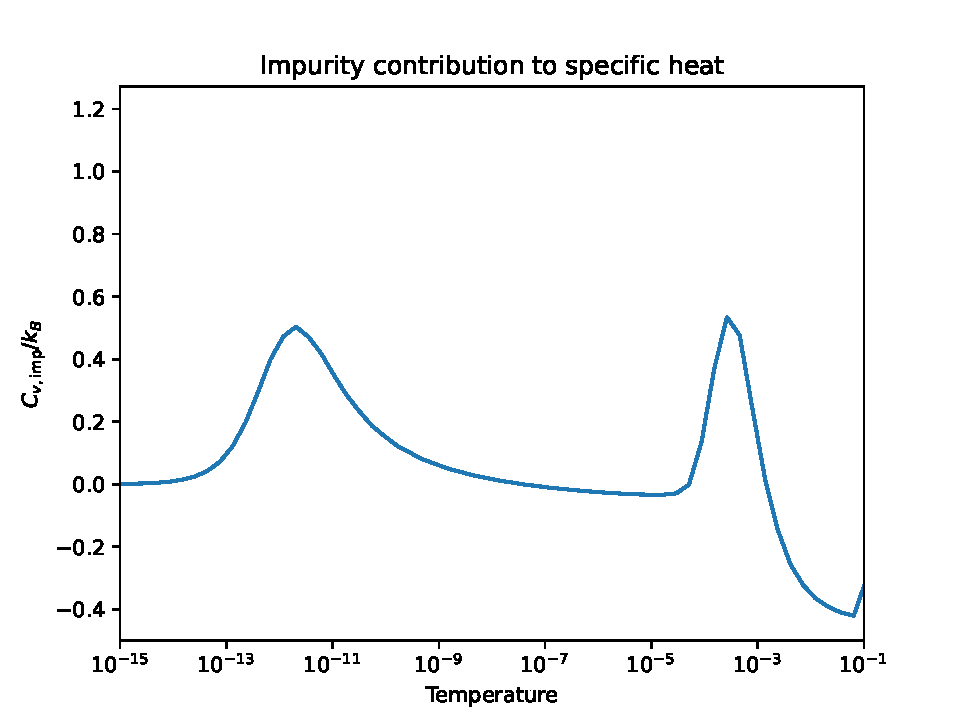
\includegraphics[width=\linewidth]{./gfx/results/Cv.pdf}
    \caption{Flow of heat capacity for $(2\epsilon_f = -U) \gg V$.}
    \label{fig:5-results-cv}
  \end{subfigure}
\end{figure}

It is definitely interesting, though, that it \textit{peaks} at the crossover points and remains roughly zero everywhere else. Perhaps this could have something to do with ``phase transitions''; of course they aren't actually phase transitions, but maybe the behavior is related.










%%% Local Variables:
%%% mode: LaTeX
%%% TeX-master: "../project"
%%% End:
